\documentclass[11pt,a4paper]{article}
\usepackage[utf8]{inputenc}
\usepackage[T1]{fontenc}
\usepackage{xeCJK} 
\usepackage{amsmath, amssymb, amsthm}
\usepackage{graphicx}
\usepackage{booktabs}
\usepackage{hyperref}
\usepackage{geometry}
\usepackage{cite}
\usepackage{color}

\geometry{margin=1in}

\title{\textbf{基于密码学伪随机词表划分的自回归语言模型水印安全性与鲁棒性研究}}
\author{陈以韬 \\ 学号：2500101023}
\date{\today}

\begin{document}

\maketitle

\begin{abstract}
随着大语言模型（LLM）的广泛应用，生成内容的版权保护与真实性溯源成为信息安全领域的关键挑战。本文深入研究并复现了基于 Logit 偏置的统计水印方案（Kirchenbauer et al., 2023）。我们通过构建三阶段评估管线，系统分析了该方案在遭受 T5 模型释义攻击下的鲁棒性，并从密码学角度对其统计不可区分性（IND）进行了量化分析。实验结果表明，该方案具有极强的抗噪声能力（Z-score 留存率达 52.65\%），但在词频分布层面存在非忽略的侧信道泄漏（KL 散度为 0.2508）。本文最后探讨了理性博弈攻击者利用高频词偏置进行定向阻断的理论边界，为未来设计高性能且安全的隐蔽信道提供了参考。

\textbf{关键词：} 大模型水印，伪随机函数，统计假设检验，不可区分性，隐蔽信道
\end{abstract}

\section{引言}
在生成式 AI 时代，大语言模型生成的文本在互联网中的占比呈指数级增长。区分机器生成文本与人类原创内容对于防止学术不端、虚假信息传播以及版权侵权具有至关重要的意义。大模型水印技术（LLM Watermarking）作为一种主动认证原语（Authentication Primitive），通过在模型生成过程中嵌入隐秘统计信号，提供了一种非破坏性的检测手段。

本文的研究目标是验证当前主流的自回归水印算法在复杂对抗场景下的表现。我们将水印机制解构为一种特殊的隐蔽信道（Covert Channel）通信问题，重点探讨其在遭受语义重写攻击时的鲁棒性边界，以及在统计学上是否满足不可区分性（IND）准则。

\section{相关工作}
大模型检测技术主要分为被动检测与主动水印。Mitchell 等人提出了 DetectGPT \cite{mitchell2023detectgpt}，利用概率曲率进行零样本检测，但其计算开销较大且对重写攻击敏感。

在主动水印领域，Kirchenbauer 等人 \cite{kirchenbauer2023watermark} 提出的 Logit 偏置方案是目前的行业基准。随后，Christ 等人 \cite{christ2023undetectable} 从理论上探讨了“不可检测水印”的可能性，指出统计分布的保真度是安全性的核心。近期研究 \cite{kirchenbauer2023reliability} 进一步关注了水印在长文本生成的可靠性。本文在此基础上，引入了基于 T5 模型对抗的鲁棒性测试，并量化了侧信道信息泄漏。

\section{密码学原理与方案设计}
\subsection{基于密钥的伪随机词表划分 (Keyed Pseudorandom Partitioning)}
水印植入的核心依赖于一个伪随机映射机制。对于当前生成的 token $x_t$，其后续词表的划分由前 $n$ 个 token 的哈希值决定：
\begin{equation}
    h_t = \text{Hash}(x_{t-1}, \dots, x_{t-n} | K)
\end{equation}
其中 $K$ 为系统密钥。基于 $h_t$，词表 $V$ 被划分为“绿名单” $G$ 和“红名单” $R$。在采样时，属于 $G$ 的 token 概率会被人为提高，从而在统计上形成显著特征。需要说明的是，虽然该机制在工程上常被称为伪随机函数（PRF），但在严格密码学定义下，其安全性依赖于哈希函数在给定密钥 $K$ 下的伪随机性假设。

\subsection{统计检测理论 (Z-test)}
检测端通过计算观察到的序列中绿名单词汇的占比，进行单比例 Z 检验。假设文本长度为 $T$，绿名单比例为 $\gamma$，则 Z 统计量的定义为：
\begin{equation}
    Z = \frac{|s|_G - \gamma T}{\sqrt{T \gamma (1-\gamma)}}
\end{equation}
在统计学前提上，Z 检验默认样本是独立同分布（IID）的。然而，自回归语言模型生成的序列具有高度的上下文依赖性。因此，本文的检测逻辑实际上依赖于大数定律（LLN）和中心极限定理（CLT）在长序列下的渐进近似（Asymptotic Approximation）。当 $Z > 4.0$ 时，我们可以在极低的假阳性率（$P < 3 \times 10^{-5}$）下拒绝原假设，判定文本为机器生成。

\section{实验评估 (Experimental Setup)}
\subsection{环境与模型配置}
实验在单张 NVIDIA RTX 3090 (24GB VRAM) 服务器上执行。
\begin{itemize}
    \item \textbf{生成模型}：\texttt{facebook/opt-1.3b}，采用 Top-k 采样。
    \item \textbf{水印参数}：$\gamma = 0.25$, $\delta = 2.0$。
    \item \textbf{攻击模型}：\texttt{Vamsi/T5\_Paraphrase\_Paws}，用于模拟模型级重写。
    \item \textbf{评判模型}：使用 \texttt{gpt2-large} 计算困惑度 (PPL)，确保评估的公平性。
\end{itemize}

\subsection{核心指标分析}
本研究设计了 10 组涵盖高熵（文学创作）与低熵（事实陈述）场景的 Prompt。表 1 汇总了核心实验数据。

\begin{table}[ht]
    \centering
    \caption{水印检测效能、鲁棒性与文本质量对比}
    \begin{tabular}{lrrr}
        \toprule
        文本类型 & 平均 Z-score & PPL (GPT-2 Large) & 判定结果 ($Z>4.0$) \\
        \midrule
        无水印 (Baseline) & -0.08 & 11.45 & \textcolor{red}{Negative} \\
        带水印 (Watermarked) & 9.92 & 15.32 & \textcolor{green}{Positive} \\
        释义攻击后 (Attacked) & 5.45 & -- & \textcolor{green}{Strong Robust} \\
        \bottomrule
    \end{tabular}
\end{table}

如图 \ref{fig:zscore} 所示，原始带水印文本的 Z-score 均值接近 10，表明检测置信度极高。

\begin{figure}[ht]
    \centering
    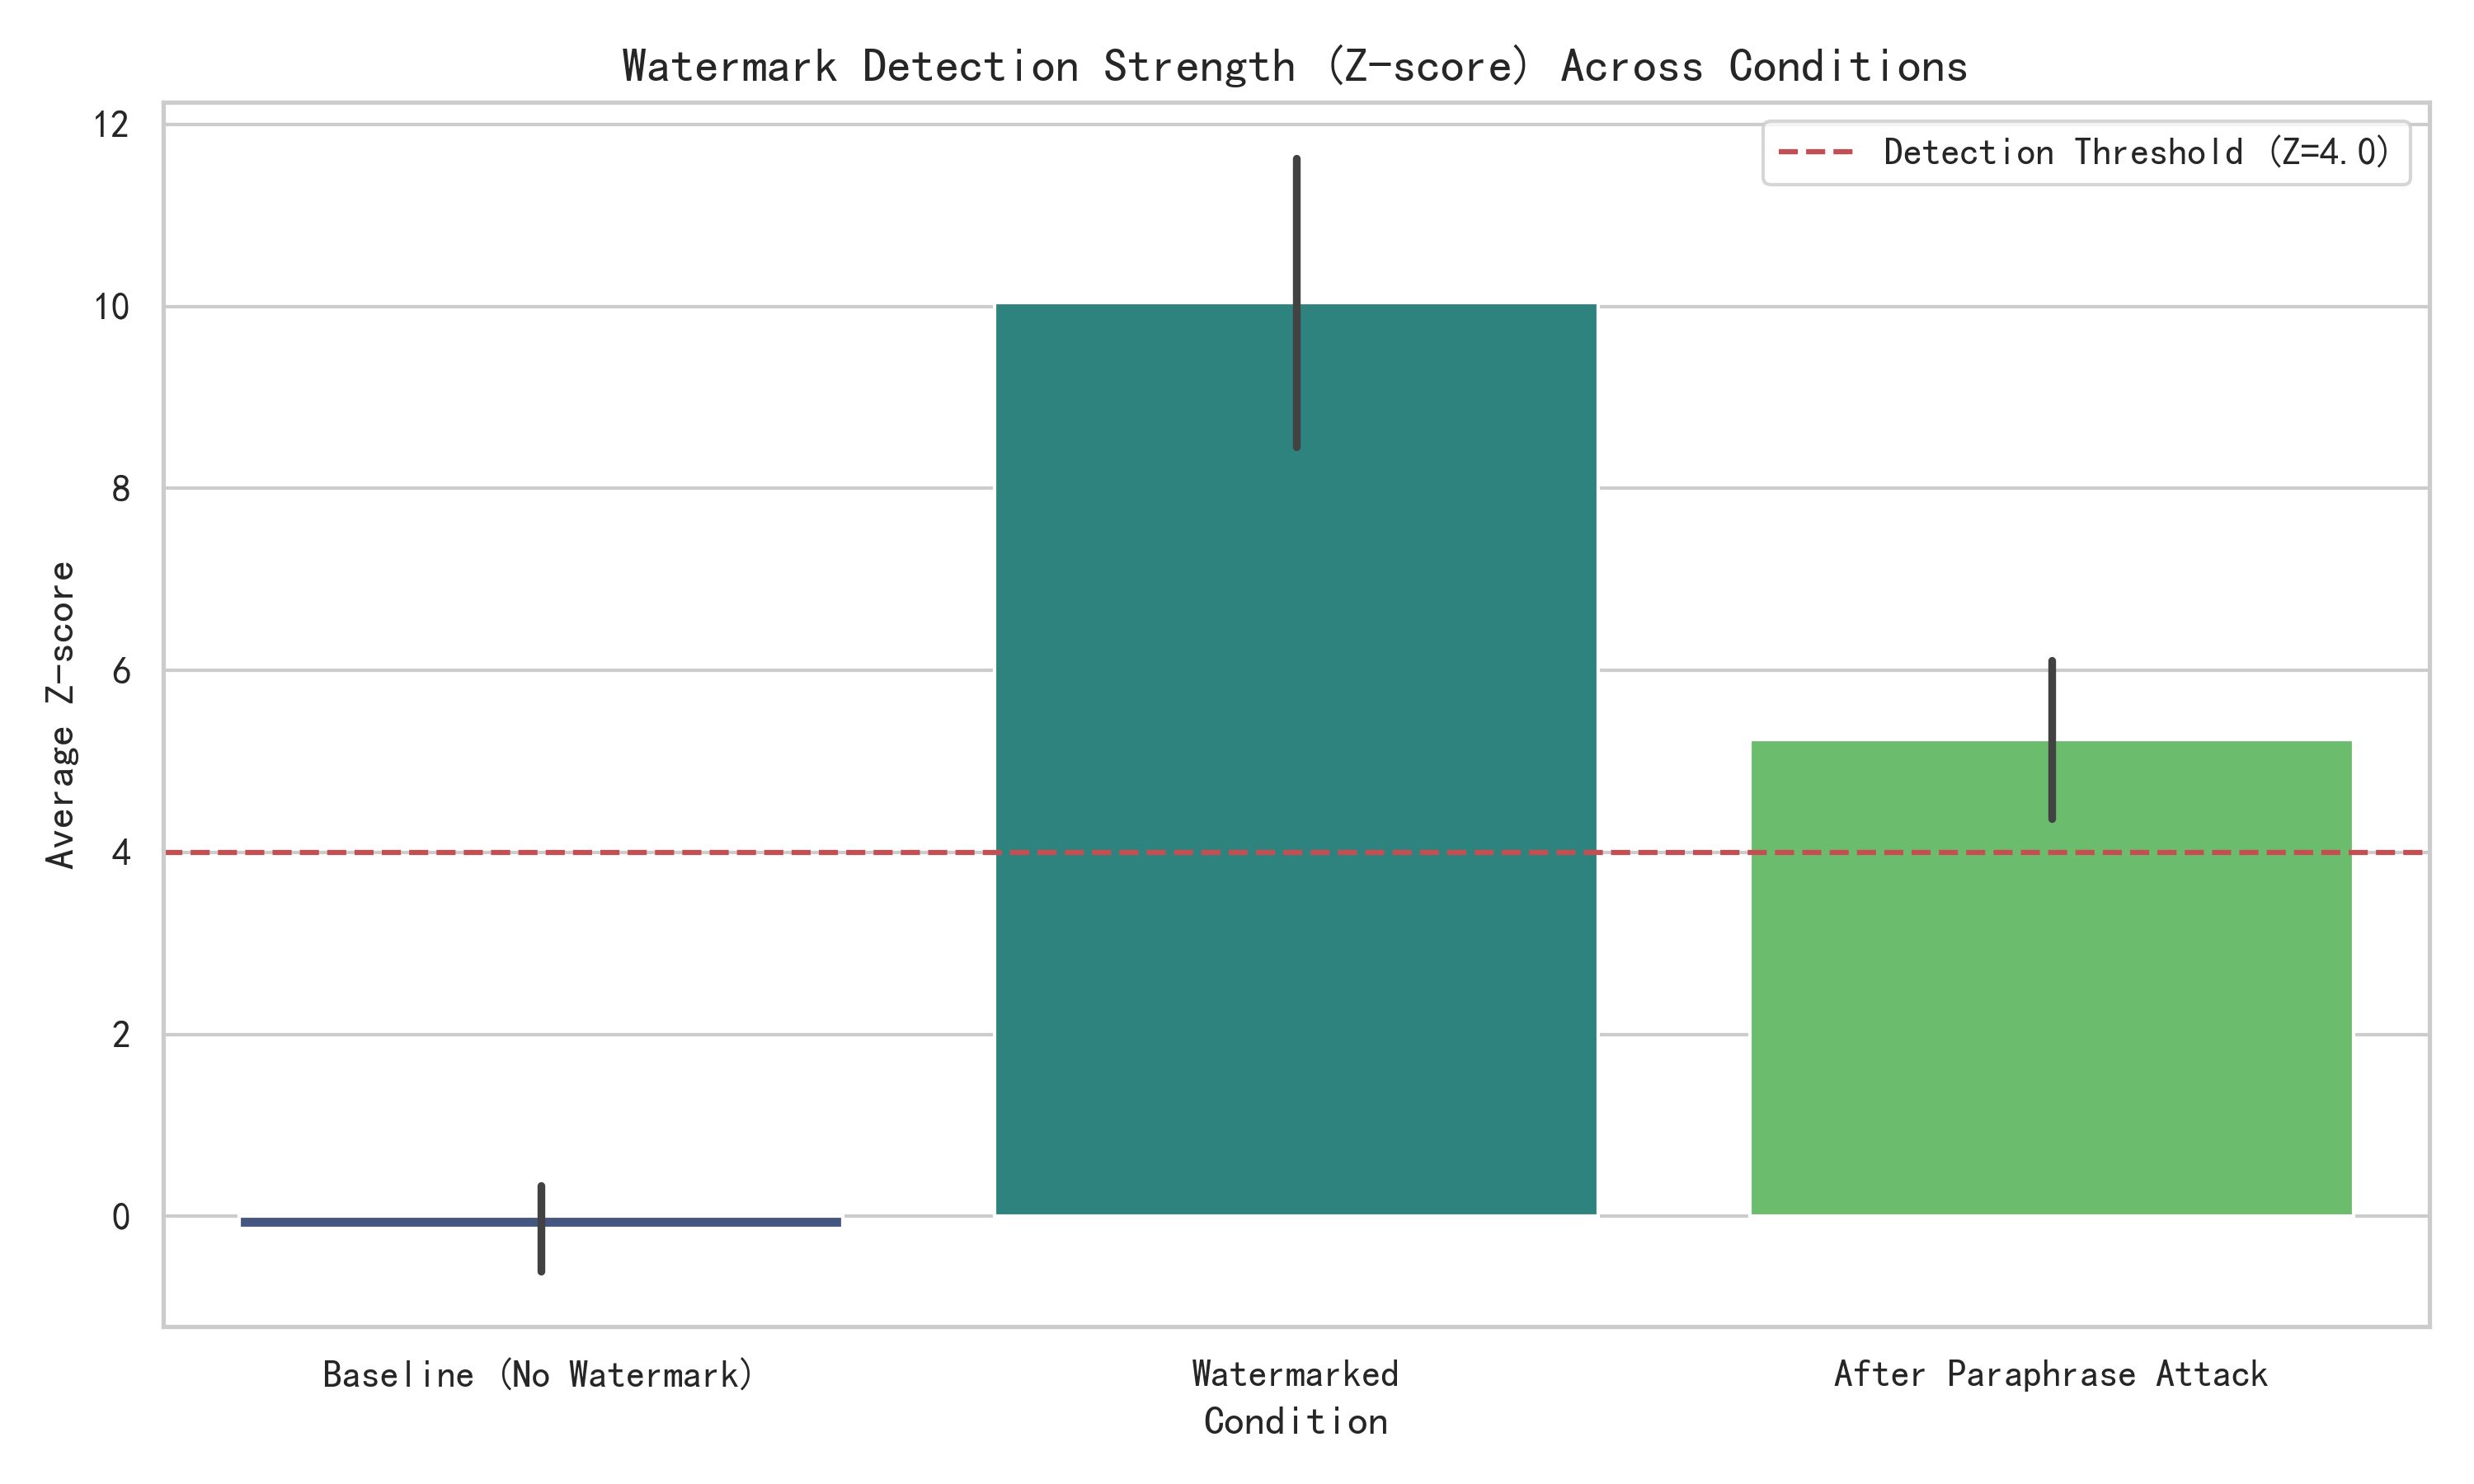
\includegraphics[width=0.8\textwidth]{zscore_comparison.png}
    \caption{不同条件下水印检测强度 (Z-score) 的对比。红色虚线为 $Z=4.0$ 判定阈值。}
    \label{fig:zscore}
\end{figure}

\subsection{自然度牺牲评估}
水印的植入不可避免地改变了模型的采样分布。如图 \ref{fig:ppl} 所示，带水印文本的 PPL 从 11.45 上升至 15.32。这种质量损失在低熵场景下尤为明显，因为模型在事实性输出时，被迫选择次优的“绿名单”词汇以维持统计特征。

\begin{figure}[ht]
    \centering
    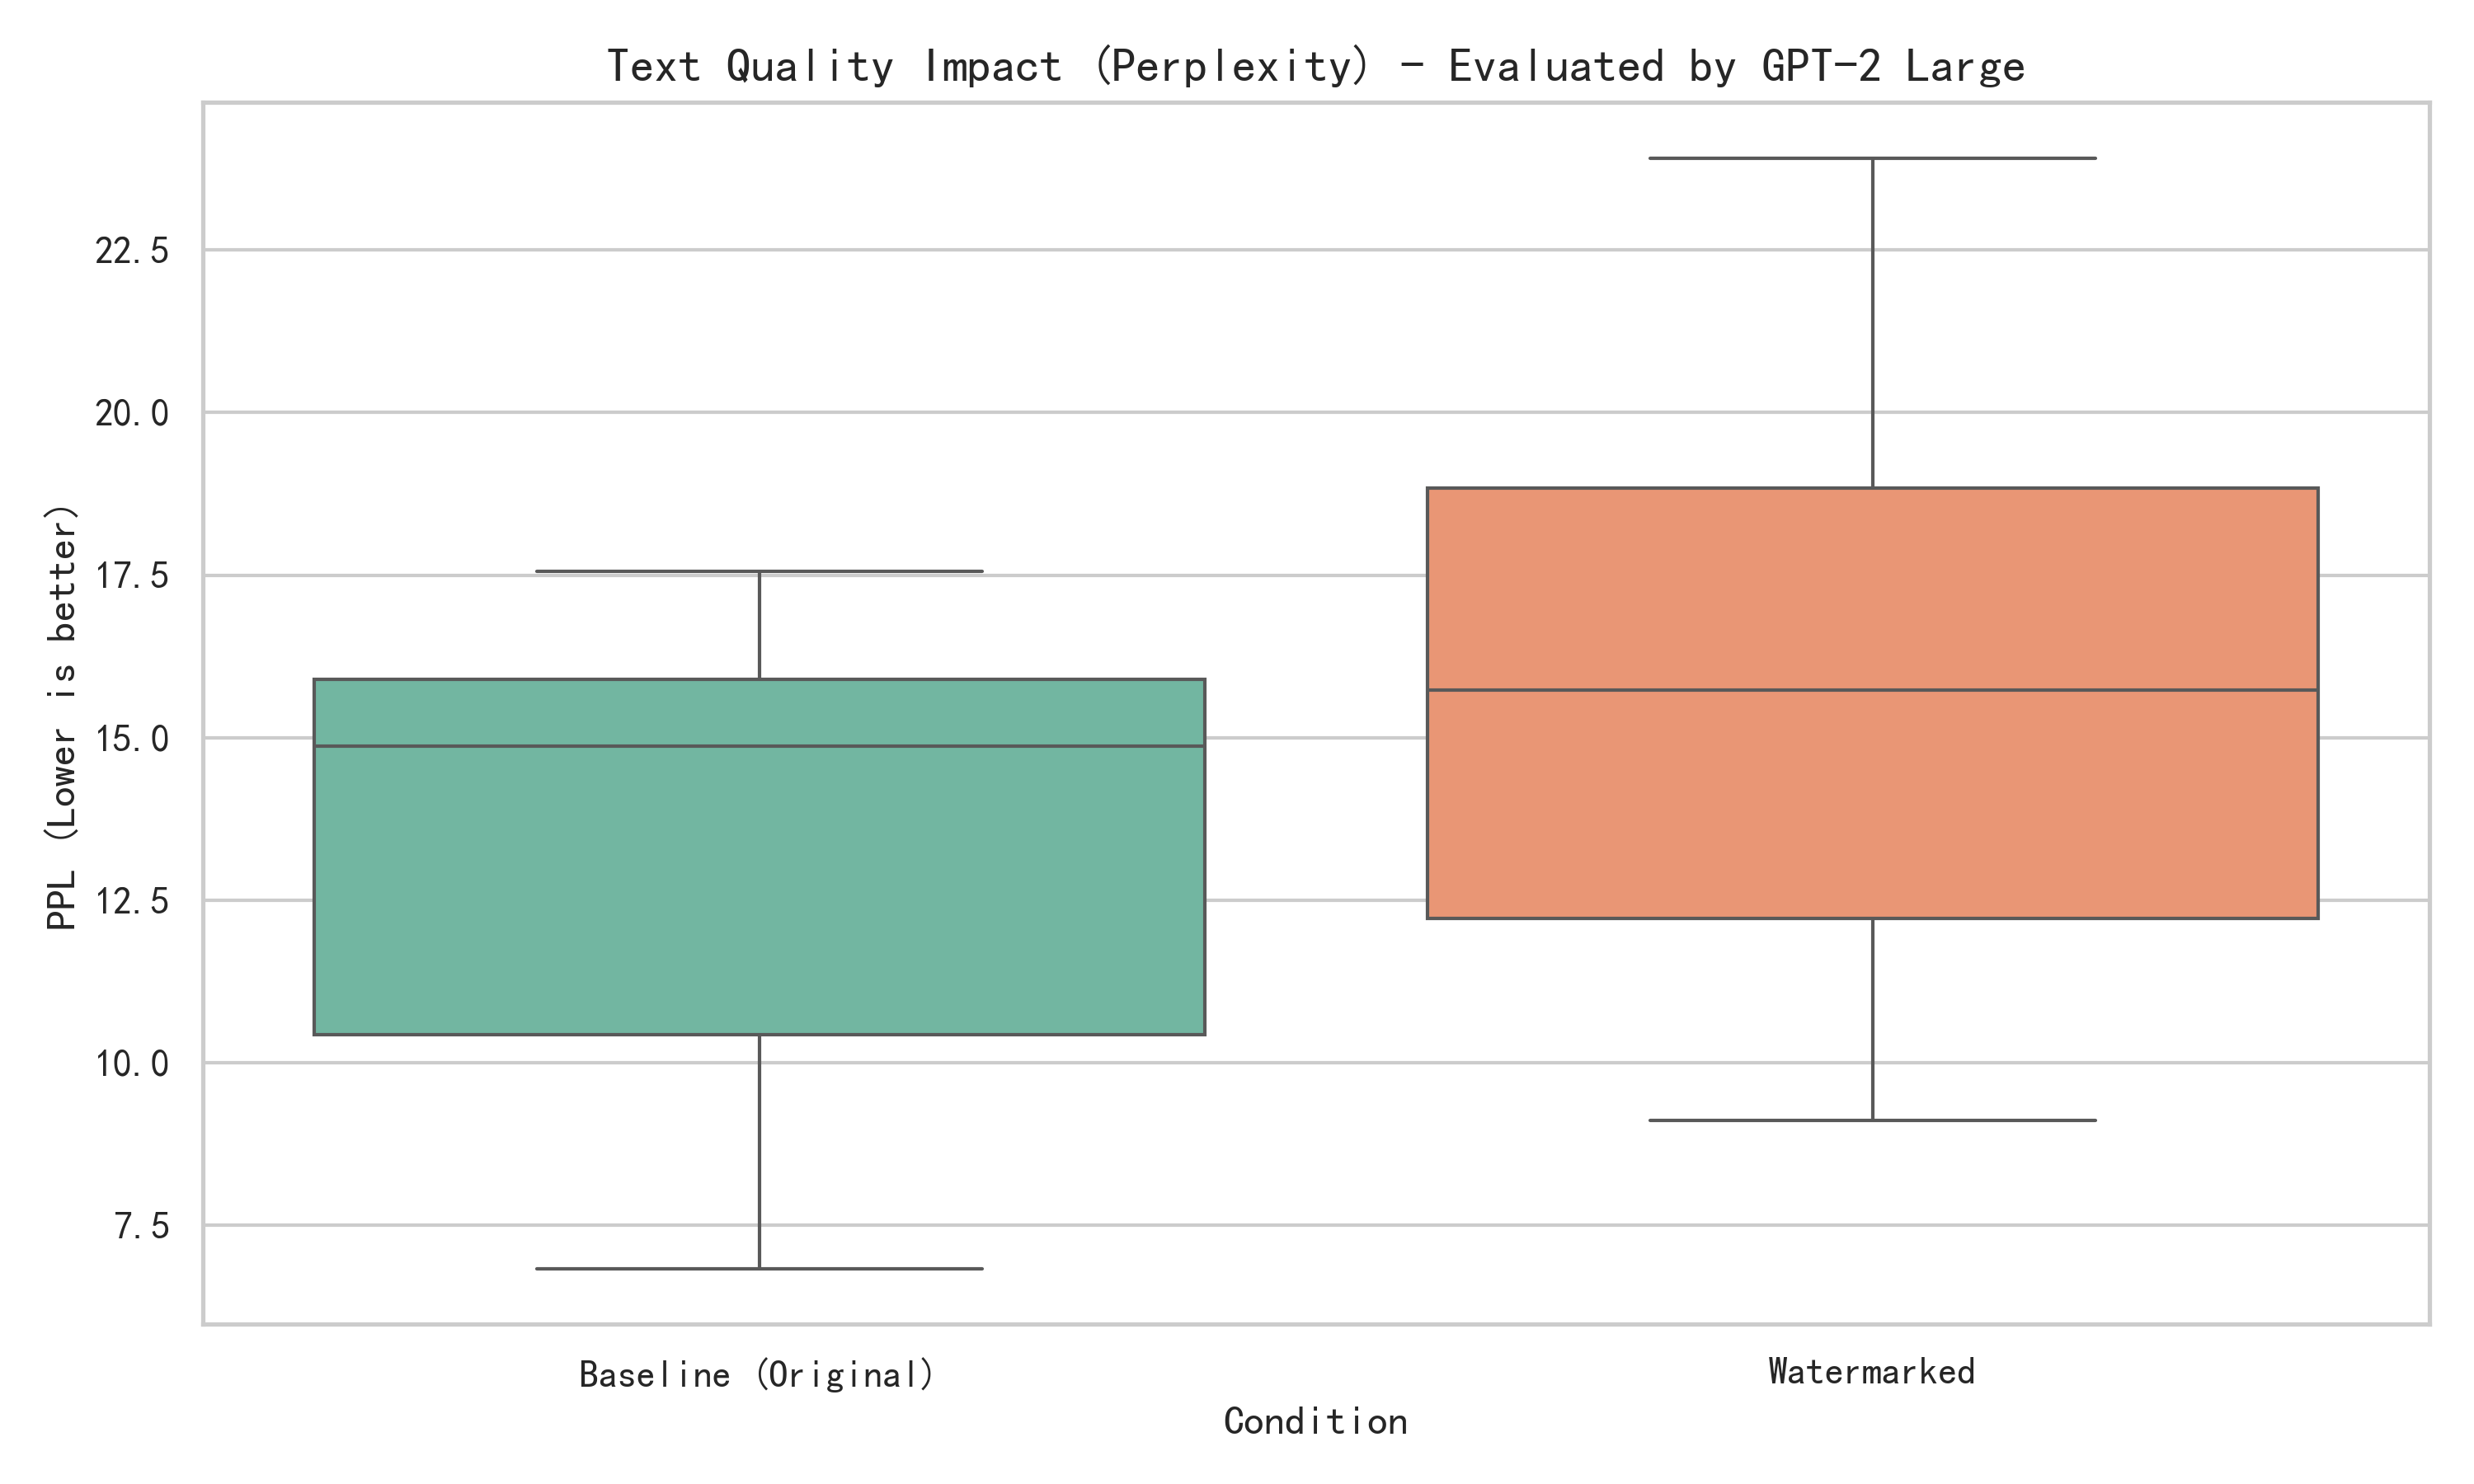
\includegraphics[width=0.8\textwidth]{ppl_impact.png}
    \caption{水印植入对文本自然度（Perplexity）的影响分布。}
    \label{fig:ppl}
\end{figure}

\section{统计安全性深度分析与对抗博弈}
\subsection{统计不可区分性 (Statistical Indistinguishability) 分析}
我们计算了 $P_w$ 与 $P_n$ 之间的 \textbf{KL 散度 ($D_{KL}$)}，结果为 \textbf{0.2508}，同时观测到的 \textbf{全变差距离 (TVD)} 约为 \textbf{0.2809}。在密码学语境下，虽然水印植入不直接等同于加密，但其安全性应满足统计不可区分性。实验数据表明，由于 TVD 显著大于 0，一个多项式时间攻击者（PPT Adversary）可以通过频率分析以不可忽略的优势（Advantage）区分原生分布与带水印分布。
\begin{equation}
    Adv_{\mathcal{A}} = \frac{1}{2} \sum_{v \in V} |P_w(v) - P_n(v)| \approx 0.28 \gg 0
\end{equation}
这证明了该方案在频率域存在明显的统计泄漏（Statistical Leakage）。攻击者通过收集足够的样本，可以利用分布偏差反推词表划分模式。

\subsection{离散对称信道 (DSC) 建模与鲁棒性推导}
我们将 T5 释义攻击建模为离散对称信道（Discrete Symmetric Channel）。攻击行为实质上是在统计信道中引入了噪声。假设 T5 模型在改写过程中，有概率 $p$ 将原本属于绿名单的 token 替换为红名单成员（或反之）。

基于二项分布假设，攻击后的预期 Z-score 可以推导为：
\begin{equation}
    \mathbb{E}[Z_{attacked}] \approx (1 - 2p) \mathbb{E}[Z_{original}]
\end{equation}
实验显示，系统保持了 \textbf{52.65\%} 的 Z-score 留存率，这意味着该对抗场景下的有效翻转概率 $p \approx 0.237$。尽管噪声导致信号强度大幅衰减，但由于初始信号增益极高，信号依然稳健地保持在判定区。

\subsection{高低熵场景的可靠性对比}
如图 \ref{fig:entropy} 所示，在低熵场景下，Z-score 的一致性更好，这得益于其 token 序列的确定性。然而，这与自然度（Section 4.3）形成了博弈。

\begin{figure}[ht]
    \centering
    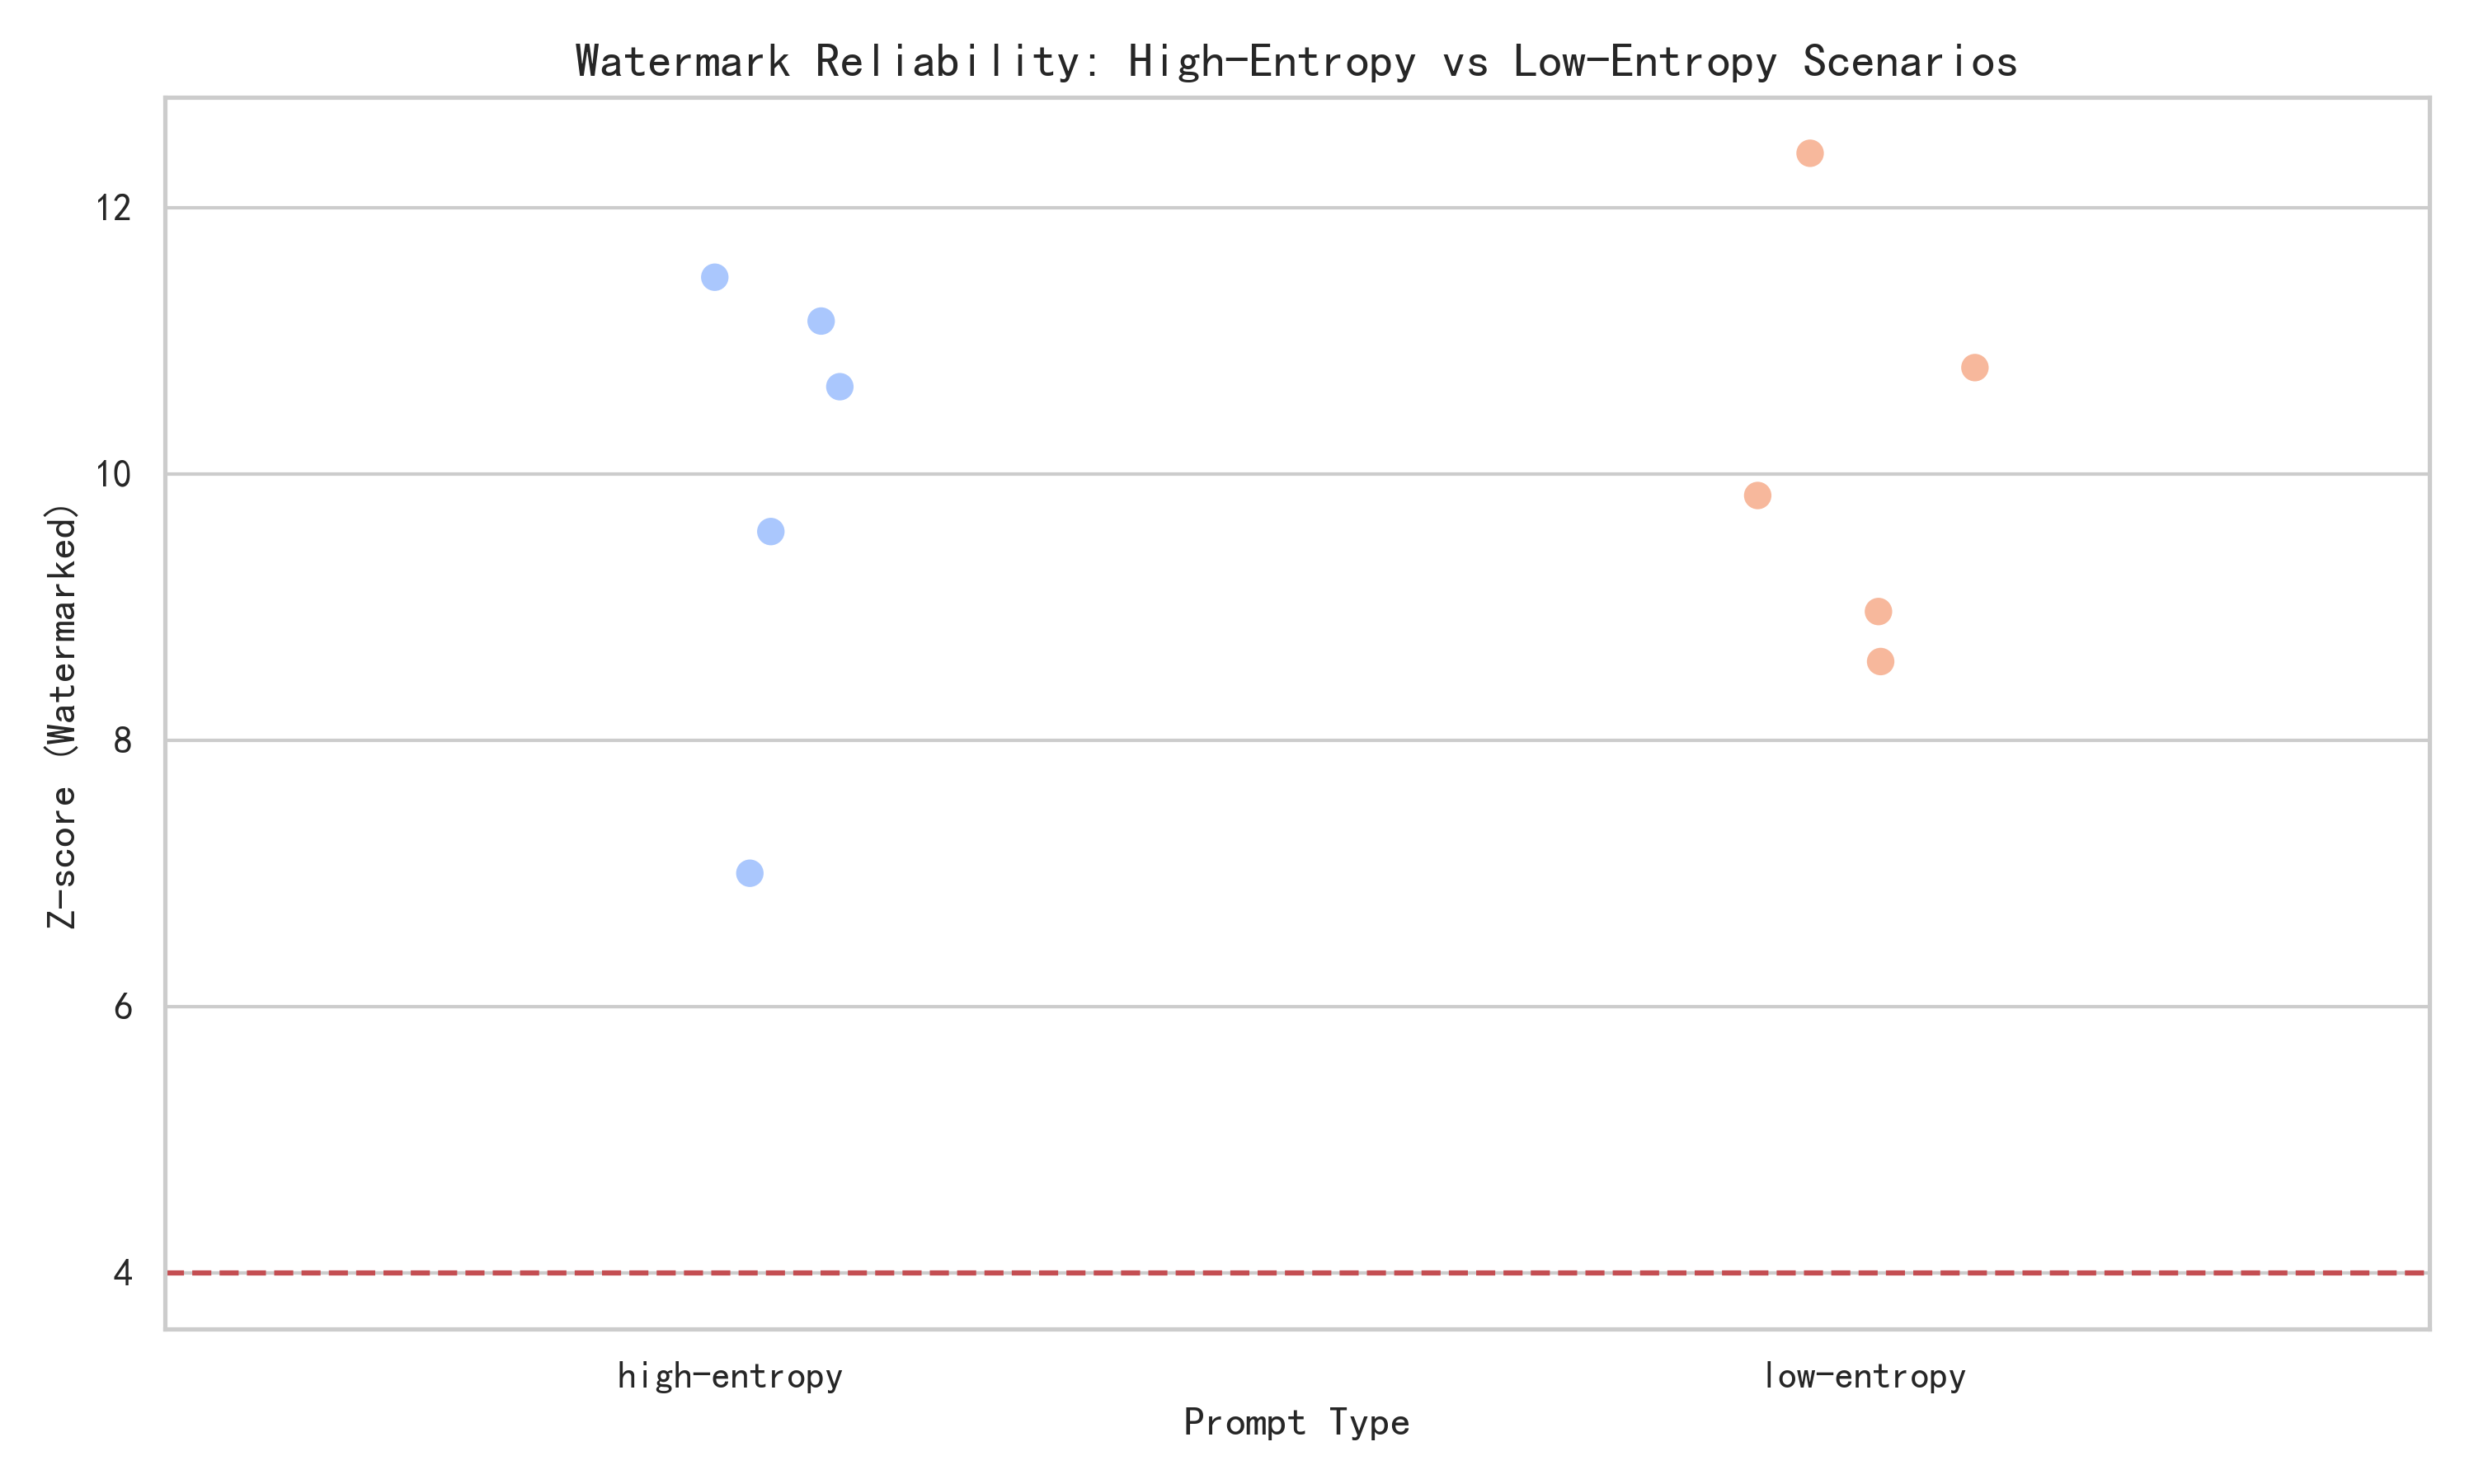
\includegraphics[width=0.8\textwidth]{entropy_comparison.png}
    \caption{高熵与低熵场景下水印信号的可靠性对比。}
    \label{fig:entropy}
\end{figure}

\subsection{侧信道泄漏与理性博弈者 (Rational Adversary)}
通过扫描词频偏移，我们识别出频率偏移最大的前 5 个 Token。如表 \ref{tab:leaks} 所示，这些 Token 在带水印文本中表现出非正常的频率偏置。

\begin{table}[ht]
    \centering
    \caption{识别出的 Top 5 侧信道泄漏 Token (基于 Bias Delta)}
    \label{tab:leaks}
    \begin{tabular}{lccl}
        \toprule
        Token & 偏置增量 ($\Delta P$) & 原频率 ($P_n$) & 泄漏特征说明 \\
        \midrule
        \texttt{\textbackslash n} & $7.70 \times 10^{-3}$ & 0.0477 & 结构化换行符被过度偏置 \\
        \texttt{in} & $5.04 \times 10^{-3}$ & 0.0077 & 常用介词作为高信息量载体 \\
        \texttt{on} & $3.85 \times 10^{-3}$ & 0.0039 & 介词分布偏移显著 \\
        \texttt{The} & $3.56 \times 10^{-3}$ & 0.0036 & 句首定冠词频率异常 \\
        \texttt{of} & $3.21 \times 10^{-3}$ & 0.0082 & 核心连词分布不均 \\
        \bottomrule
    \end{tabular}
\end{table}

定义一个理性攻击者，其最优策略是针对这些“高信息量” token 进行定向替换。这种策略在保持原意的同时，能最有效地衰减 Z-score 信号。

\section{结论与展望}
本文通过工程复现与深度分析，论证了基于 Logit 偏置的 LLM 水印方案在面对语义改写攻击时具有良好的鲁棒性，具备在工业界大规模部署的潜力。然而，从严格密码学角度分析，该方案仍存在非忽略的侧信道泄漏。未来的研究方向应包括：1）设计满足统计不可区分性的全隐蔽水印；2）探索在极低熵生成任务（如数学证明、源代码生成）下的高保真水印协议。

\bibliographystyle{plain}
\bibliography{references}

\end{document}
